\documentclass[italian,12pt]{article}

\def\Title{Verbale interno}
\def\Subtitle{Riunione interna settimanale}
\def\Author{7Last}
\def\Date{2024-05-22}
\def\Version{v1.0}

%pacchetti extra da scaricare dblfloatfix, fancyhdr
\usepackage[left=2cm, right=2cm, bottom=3cm, top=3cm]{geometry}
\usepackage{fancyhdr}%creazione header-footer
\usepackage{graphicx} %serve per inserire immagini
\graphicspath{ {../../../logo/} }
%\usepackage{dblfloatfix} %serve per posizionare gli elementi dove si vuole
\usepackage[hidelinks]{hyperref} %serve per i link
\usepackage{tikz}
\usepackage{tgadventor} % font
\usepackage[useregional=numeric,showseconds=true,showzone=false]{datetime2}
\usepackage{caption}

\usepackage{hyperref}
\usepackage{tocloft}
\usepackage{titlesec}
\usepackage{color}
\usepackage{ulem}
\usepackage{pgfplots}
\usepackage{pgf-pie}
\usepackage[italian]{babel}
\usepackage{comment}
\usepackage{tabularx}
\usepackage{longtable}
\usepackage{float}
\usepackage{amsmath}

\linespread{1.2}
\captionsetup[table]{name=Tabella}
\geometry{headsep=1.5cm}

\renewcommand{\contentsname}{Indice}
\renewcommand\familydefault{\sfdefault}
\renewcommand{\listtablename}{Indice delle tabelle}
\renewcommand\familydefault{\sfdefault}
\renewcommand{\listfigurename}{Indice delle immagini}
\renewcommand\familydefault{\sfdefault}

% set sfdefault for page numbers
\let\oldthepage\thepage
\renewcommand{\thepage}{\sffamily\oldthepage}

\begin{document}
\newgeometry{left=2cm,right=2cm,bottom=2.1cm,top=2.1cm}
\begin{titlepage}
    \vspace*{.5cm}

    \vspace{2cm}
    {
        \centering
        {\bfseries\huge \Title\par}
        \bigbreak
        {\bfseries\large \Author\par}
        \bigbreak
        {\Version\par}
        \vfill

        \begin{tikzpicture}[remember picture,overlay]

            \fill[blue!20!black] (current page.south west) -- ++(10cm,0) -- ++(-10cm,15cm) -- cycle;
            \fill[orange] (current page.south east) -- ++(-18cm,0) -- ++(21.6cm,22cm) -- cycle;

            \clip (0,-3cm) circle (2.5cm) node (current page.center) {
\includegraphics[width=5cm]{logo.jpg}};
        \end{tikzpicture}

    }

    \vfill

\end{titlepage}

\restoregeometry





















\newpage
%---------------header------------------%
\pagestyle{fancy}
\fancyhead{} % pulizia degli header
\lhead{%
\begin{tikzpicture}
    \clip (0,0) circle (0.5cm);
    \node at (0,0) {
\includegraphics[width=1cm]{logo}};
\end{tikzpicture}%
}
\chead{\vspace{\fill}\Title\vspace{\fill}}
\rhead{\vspace{\fill}\Version\vspace{\fill}}
%quad è una spaziatura
%---------------------------------------%

\begin{table}[!h]
	\caption*{Versioni}
	\begin{center}
		\begin{tabular}{ c c c c p{6.1cm} }
			\hline                                                                                                 \\[-2ex]
			Ver. & Data       & Redattore     & Verificatore      & Descrizione                                    \\
			\\[-2ex] \hline \\[-1.5ex]
			1.0  & 2024-04-23 & Elena Ferro   & Antonio Benetazzo & Aggiunte conclusioni                           \\
			0.3  & 2024-04-23 & Elena Ferro   & Antonio Benetazzo & Correzioni e aggiunte                          \\
			0.2  & 2024-04-22 & Matteo Tiozzo & Antonio Benetazzo & Benchmark, Tabella riassuntiva                 \\
			0.1  & 2024-04-22 & Elena Ferro   & Antonio Benetazzo & Vantaggi di Redpanda, Vantaggi di Apache Kafka \\
			\\[-1.5ex] \hline
		\end{tabular}
	\end{center}
\end{table}

\newpage
\tableofcontents
\listoftables
\listoffigures
\newpage

\section{Introduzione}
\subsection{Obiettivo del documento}
Il presente documento ha lo scopo di definire le strategie di verifica e validazione utilizzate per assicurare il corretto funzionamento dello strumento sviluppato e delle
attività che lo accompagnano.  Sarà sottoposto a revisioni continue, così da prevedere situazioni precedentemente non occorse e da seguire l'evoluzione del progetto.
\subsection{Glossario}
Il \href{https://7last.github.io/docs/rtb/documentazione-interna/glossario#glossario}{glossario\textsubscript{G}} è uno strumento utilizzato per risolvere eventuali dubbi riguardanti 
alcuni termini specifici utilizzati nella redazione del documento.
Esso conterrà la definizione dei termini evidenziati e sarà consultabile al seguente \href{https://7last.github.io/docs/rtb/documentazione-interna/glossario}{link}. I termini presenti in tale documento saranno evidenziati da una 'G' a pedice.
\subsection{Riferimenti}
\subsubsection{Riferimenti normativi}
\begin{itemize}
    \item \href{https://7last.github.io/docs/rtb/documentazione-interna/glossario#norme-di-progetto}{Norme di progetto\textsubscript{G}} (aggiungere versione e/o link al documento);
    \item Regolamento del progetto:\\
		  \url{https://www.math.unipd.it/~tullio/IS-1/2023/Dispense/PD2.pdf}.
\end{itemize}
\subsubsection{Riferimenti informativi}
\begin{itemize}
    \item \href{https://7last.github.io/docs/rtb/documentazione-interna/glossario#capitolato}{Capitolato\textsubscript{G}} d'appalto C6: \href{https://7last.github.io/docs/rtb/documentazione-interna/glossario#synccity}{SyncCity\textsubscript{G}} – A \href{https://7last.github.io/docs/rtb/documentazione-interna/glossario#smart-city}{smart city\textsubscript{G}} monitoring platform\\
    \url{https://www.math.unipd.it/~tullio/IS-1/2023/Progetto/C6.pdf};
    \item \href{https://it.wikipedia.org/wiki/ISO/IEC_9126}{Standard ISO/IEC 9126};
    \item \href{https://iso25000.com/index.php/en/iso-25000-standards/iso-25010}{Standard ISO/IEC 25010};
    \item \href{ https://en.wikipedia.org/wiki/ISO/IEC_12207}{Standard ISO/IEC 12207:1995};
    \item \href{URL}{\textit{Verbali esterni}};
    \item \href{URL}{\textit{Verbali interni}};
    \item \href{URL}{\href{https://7last.github.io/docs/rtb/documentazione-interna/glossario#analisi-dei-requisiti}{\textit{Analisi dei requisiti}\textsubscript{G}}};
    \item AGGIUNGERE LINK
\end{itemize}

\section{Vantaggi di Redpanda}
\subsection{Performance}
Redpanda è scritto in C++ e utilizza il \textit{framework} Seastar, offrendo un'architettura \textit{thread-per-core} ad alte prestazioni.
Ciò permette di ottenere un'elevata \textit{throughput} e latenze costantemente basse, evitando cambi di contesto e blocchi.
Inoltre, è progettato per sfruttare l'\textit{hardware} moderno, tra cui unità NVMe, processori \textit{multi-core} e interfacce di rete ad alta velocità.

\subsection{Costi}
Anche per carichi di lavoro ridotti, l'utilizzo di Kafka può essere \href{https://redpanda.com/blog/is-redpanda-better-than-kafka-tco-comparison}{fino a 3 volte più costoso} rispetto a Redpanda. Per carichi di lavoro più complessi, questa differenza può aumentare fino a 5 volte o più.

\subsection{Semplicità di configurazione}
Il binario di Redpanda include, oltre al \textit{message broker}, anche
un \textit{proxy} HTTP e uno \textit{schema registry}.

\subsection{BYOC (\textit{Bring Your Own Cluster})}
Redpanda offre una terza opzione oltre alla gestione autonoma di un \textit{cluster} di \textit{streaming}
dati e all'utilizzo di un servizio \textit{cloud} completamente gestito: \textit{Bring Your Own Cluster} (BYOC).
Questa alternativa consente agli utenti finali di implementare una soluzione parzialmente gestita dal fornitore nella propria infrastruttura (come il proprio \textit{data center}
o il proprio \textit{VPC cloud}).

\subsection{Compatibilità con API di Kafka}
Redpanda è progettato per essere compatibile con le API di Kafka, consentendo di utilizzare i \textit{client} Kafka esistenti senza modifiche.

\subsection{\textit{Self-healing}}
Redpanda è self-healing e redistribuisce continuamente i dati e la \textit{leadership} tra i nodi per mantenere il \textit{cluster} in uno stato ottimale mentre il \textit{cluster} evolve o quando i nodi falliscono.


\begin{center}
	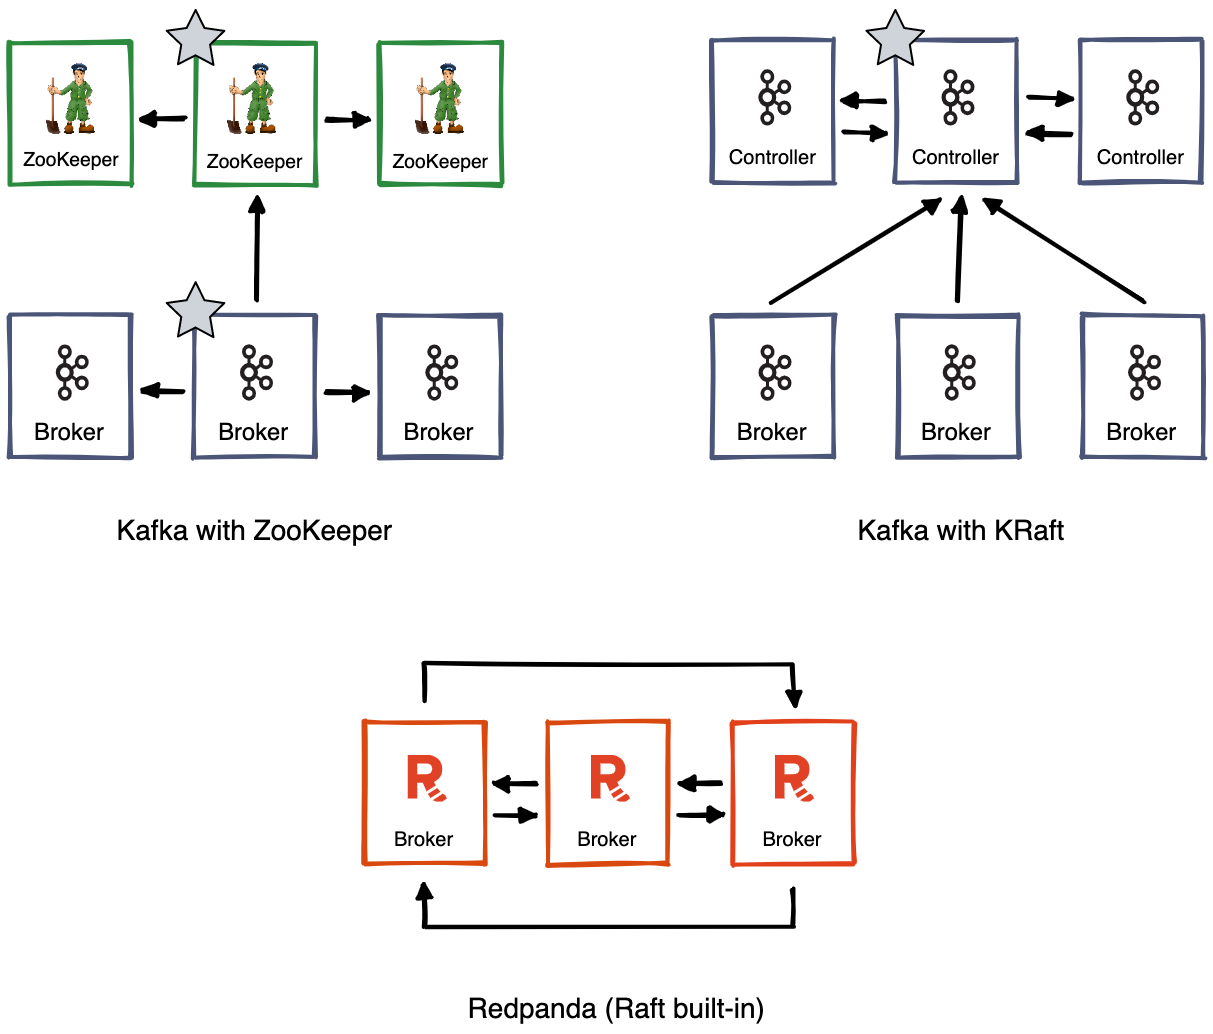
\includegraphics[width=0.65\textwidth]{imgs/kafka_zookeeper.png}
	\captionof{figure}{\href{https://redpanda.com/blog/kafka-kraft-vs-redpanda-performance-2023}{Architettura di Kafka con ZooKeeper}}
\end{center}














\section{Vantaggi di Apache Kafka}
\subsection{Maturità}
Redpanda è stato rilasciato per la prima volta nel 2019, mentre \href{https://7last.github.io/docs/rtb/documentazione-interna/glossario\#apache-kafka}{Apache Kafka\textsubscript{G}} nel 2011.
Quest'ultimo dunque ha potuto svilupparsi e stabilizzarsi nel tempo, raggiungendo
un livello di maturità più elevato rispetto a Redpanda.\\
Ne consegue dunque che Kafka è maggiormente diffuso e utilizzato in ambienti di
produzione.

\subsection{Licenza}
\href{https://7last.github.io/docs/rtb/documentazione-interna/glossario\#apache-kafka}{Apache Kafka\textsubscript{G}} è rilasciato con la licenza \textit{open source} Apache 2.0, la quale consente di utilizzare, modificare e distribuire il software liberamente.
Al contrario, sia l'edizione \textit{community} che quella \textit{enterprise} di Redpanda hanno licenza Business Source License (BSL), che
nonostante renda il codice sorgente disponibile, impone delle restrizioni sull'utilizzo e la distribuzione del software.


\subsection{Comunità e supporto}
Kafka ha una vasta e attiva comunità di sviluppatori, che forniscono supporto, risorse e strumenti per estendere e migliorare il progetto.
La sua documentazione è molto completa e ben strutturata, con numerosi tutorial, guide e risorse online per imparare ad utilizzarlo.\\
Redpanda al contrario ha una comunità più piccola e meno attiva, con un numero ridotto di risorse disponibili.

\subsection{Integrazione con altri servizi}
Kafka è supportato da una vasta gamma di strumenti e librerie di terze parti che lo integrano con altri sistemi e servizi
(con cui tuttavia \href{https://docs.redpanda.com/current/develop/kafka-clients/}{Redpanda è compatibile}).

\subsection{Scalabilità}
Redpanda dimostra bassa latenza e alto throughput su \textit{workload} semplici. Tuttavia esso è stato studiato per essere ottimizzato per il \textit{random IO}, e non per il \textit{sequential IO} come Kafka.\\
Questo significa che in situazioni con un alto numero di produttori, un utilizzo del disco superiore al 30\%, l'abilitazione delle chiavi dei messaggi, l'abilitazione di TLS o l'esecuzione per più di 24 ore,
le prestazioni di Redpanda possono degradarsi significativamente.\\

\subsection{Protocollo di replicazione}
Il protocollo Raft utilizzato da Redpanda per la replicazione e la scrittura su disco è sincrona. \\
Nei sistemi Linux \textit{fsync} garantisce che i dati siano persistiti in modo sincrono, tuttavia
è un'operazione costosa in termini di prestazioni.\\
\href{https://7last.github.io/docs/rtb/documentazione-interna/glossario\#apache-kafka}{Apache Kafka\textsubscript{G}} può essere configurato per utilizzare anche un protocollo di replicazione asincrono, che non richiede l'utilizzo di \textit{fsync}.
Nonostante ciò, Redpanda è in grado di garantire prestazioni migliori rispetto a Kafka, come mostrato nel grafico sottostante.

\begin{center}
	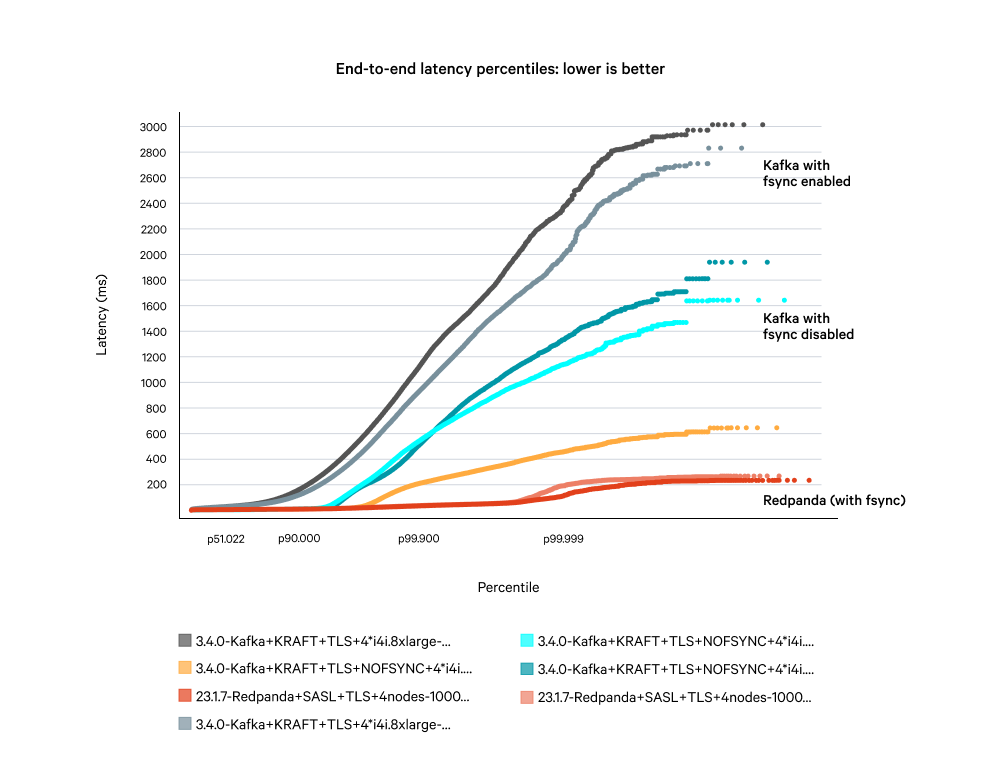
\includegraphics[width=0.75\textwidth]{imgs/fsync.png}
	\captionof{figure}{\href{https://redpanda.com/blog/kafka-kraft-vs-redpanda-performance-2023}{Confronto di latenza tra Kafka e Redpanda con e senza \textit{fsync}.}}
\end{center}






























\section{\textit{Benchmark}}
Seguono i risultati dei \textit{benchmark} effettuati dal team di sviluppo di TimescaleDB, che confrontano
le prestazioni dei due strumenti.

\begin{center}
	\includegraphics[width=0.85\textwidth]{imgs/01-timescale-vs-\href{https://7last.github.io/docs/pb/documentazione-interna/glossario\#clickhouse}{clickhouse\textsubscript{G}}.png}
	\captionof{figure}{\href{https://www.timescale.com/blog/what-is-clickhouse-how-does-it-compare-to-postgresql-and-timescaledb-and-how-does-it-perform-for-time-series-data/}{\href{https://7last.github.io/docs/pb/documentazione-interna/glossario\#clickhouse}{ClickHouse\textsubscript{G}} ha performance migliori di TimescaleDB con batch di dimensione superiore a 5,000 righe}}
\end{center}

\begin{center}
	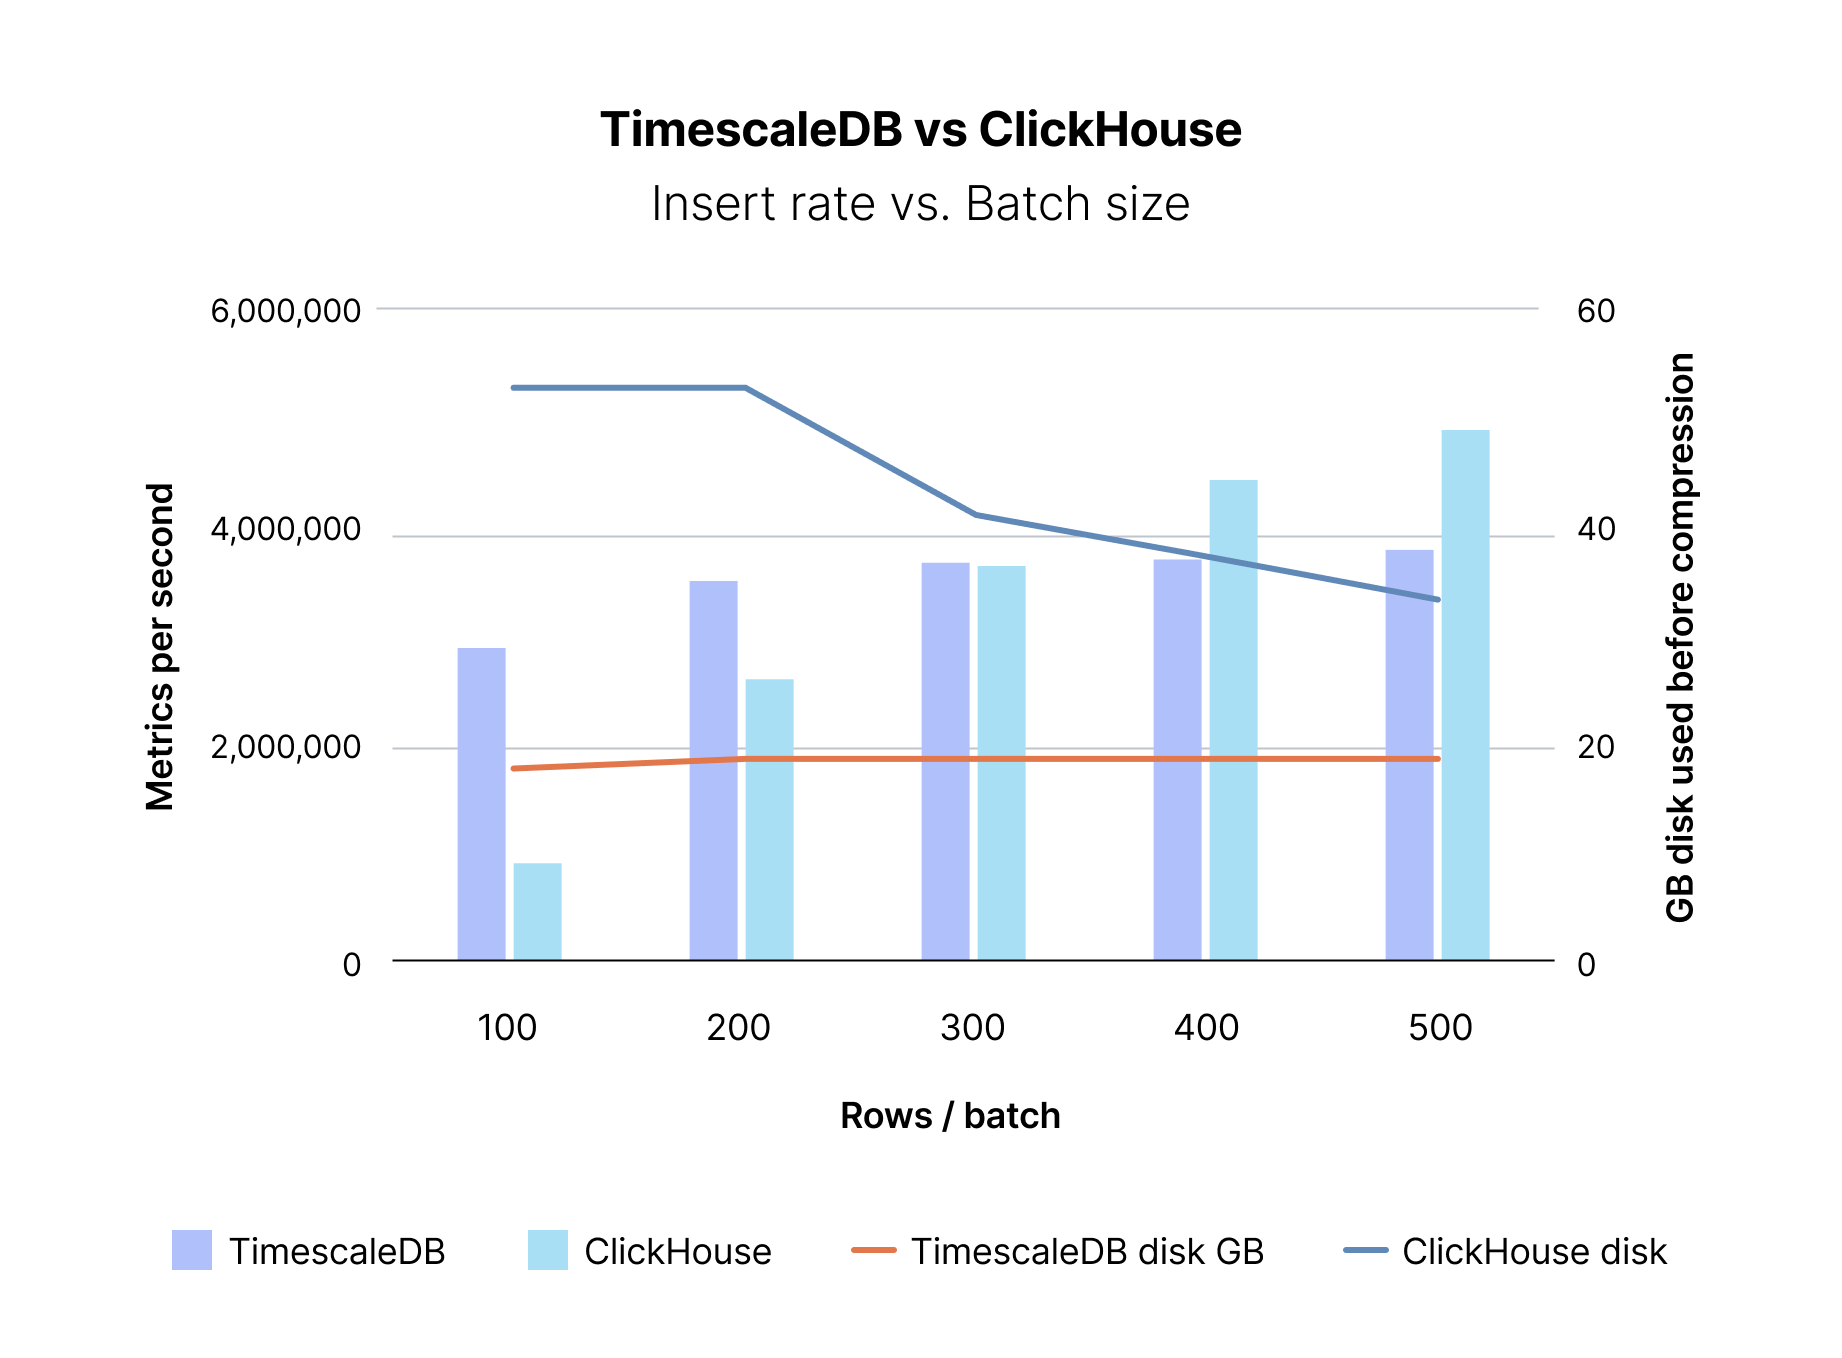
\includegraphics[width=0.85\textwidth]{imgs/02-small-batch-insert-performance.png}
	\captionof{figure}{\href{https://www.timescale.com/blog/what-is-clickhouse-how-does-it-compare-to-postgresql-and-timescaledb-and-how-does-it-perform-for-time-series-data/}{Timescale ha performance migliori di \href{https://7last.github.io/docs/pb/documentazione-interna/glossario\#clickhouse}{ClickHouse\textsubscript{G}} con batch di dimensione più contenuta e usa una quantità di disco inferiore di 2.7 volte}}
\end{center}

\begin{center}
	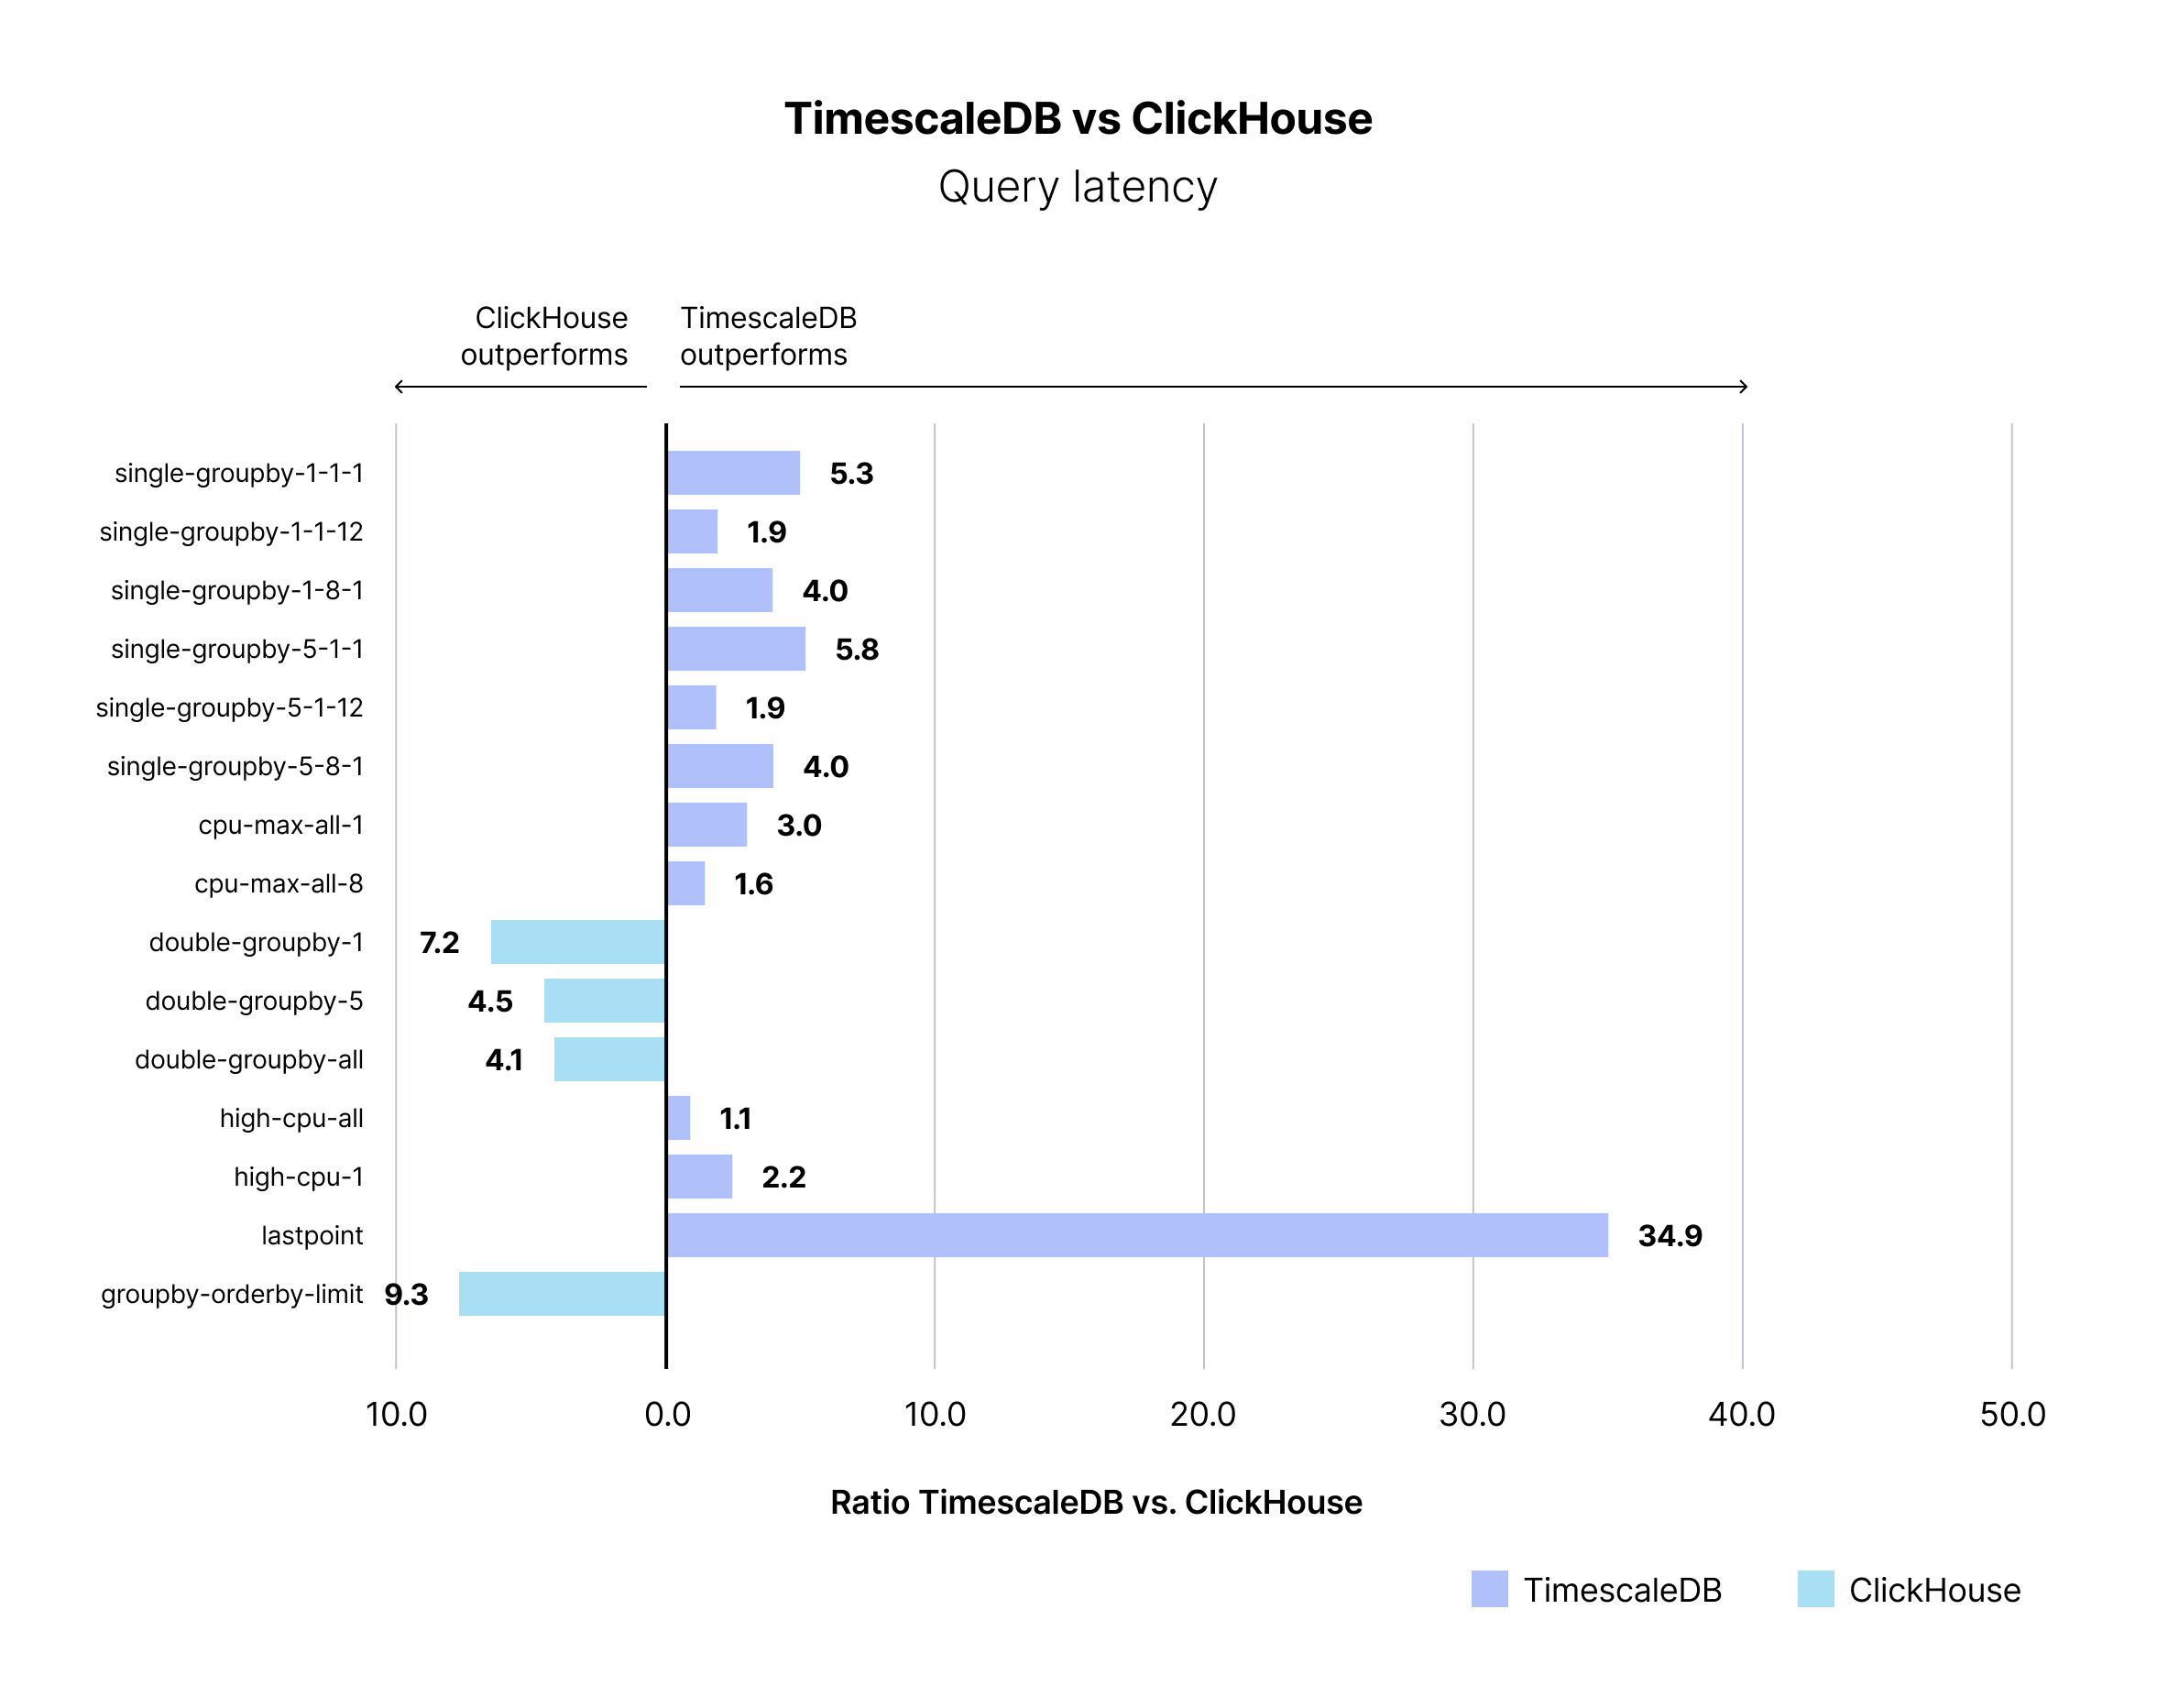
\includegraphics[width=0.85\textwidth]{imgs/03-query-latency.png}
	\captionof{figure}{\href{https://www.timescale.com/blog/what-is-clickhouse-how-does-it-compare-to-postgresql-and-timescaledb-and-how-does-it-perform-for-time-series-data/}{Performance relative alle query}}
\end{center}

\begin{center}
	\includegraphics[width=0.85\textwidth]{imgs/07-\href{https://7last.github.io/docs/pb/documentazione-interna/glossario\#clickhouse}{clickhouse\textsubscript{G}}-improvement.png}
	\captionof{figure}{\href{https://www.timescale.com/blog/what-is-clickhouse-how-does-it-compare-to-postgresql-and-timescaledb-and-how-does-it-perform-for-time-series-data/}{Performance degli insert}}
\end{center}

\begin{center}
	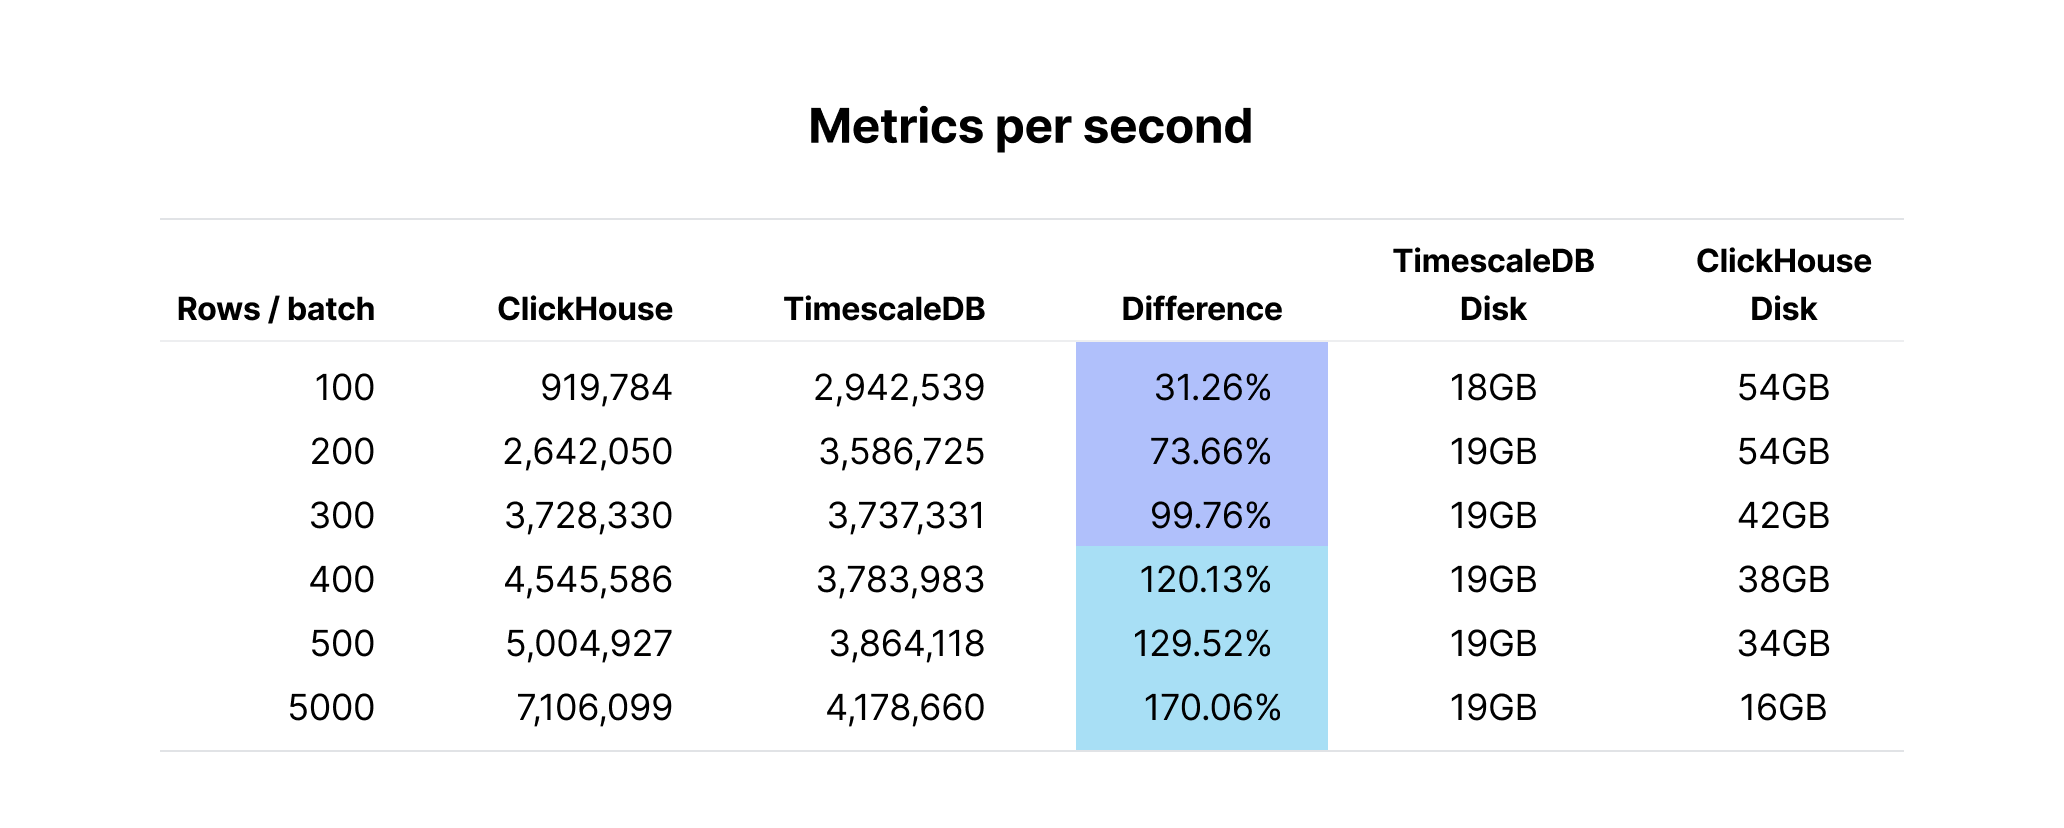
\includegraphics[width=0.85\textwidth]{imgs/08-chunk-time-interval.png}
	\captionof{figure}{\href{https://www.timescale.com/blog/what-is-clickhouse-how-does-it-compare-to-postgresql-and-timescaledb-and-how-does-it-perform-for-time-series-data/}{Performance degli insert con batch di dimensioni ridotte}}
\end{center}

\begin{center}
	\includegraphics[width=0.85\textwidth]{imgs/09-\href{https://7last.github.io/docs/pb/documentazione-interna/glossario\#clickhouse}{clickhouse\textsubscript{G}}-benchmark-read-latency-performance.png}
	\captionof{figure}{\href{https://www.timescale.com/blog/what-is-clickhouse-how-does-it-compare-to-postgresql-and-timescaledb-and-how-does-it-perform-for-time-series-data/}{Performance di query di 4000 host con 100 milioni di righe di dati}}
\end{center}

\begin{center}
	\includegraphics[width=0.85\textwidth]{imgs/10-\href{https://7last.github.io/docs/pb/documentazione-interna/glossario\#clickhouse}{clickhouse\textsubscript{G}}-benchmark-read-latency-performance.png}
	\captionof{figure}{\href{https://www.timescale.com/blog/what-is-clickhouse-how-does-it-compare-to-postgresql-and-timescaledb-and-how-does-it-perform-for-time-series-data/}{Performance di query di 10000 host con 100 milioni di righe di dati}}
\end{center}








\section{Tabella riassuntiva}

\begin{longtable}{|>{\centering\arraybackslash}p{0.30\textwidth}|>{\centering\arraybackslash}p{0.30\textwidth}|>{\centering\arraybackslash}p{0.30\textwidth}|}
	\hline
	\textbf{Paragone}                    & \textbf{Apache Kafka}                                                                                                                                       & \textbf{Redpanda}                                                                                                                                                                \\
	\hline
	\endfirsthead
	\hline
	\textbf{Paragone}                    & \textbf{Apache Kafka}                                                                                                                                       & \textbf{Redpanda}                                                                                                                                                                \\
	\endhead
	\hline
	\textbf{Adozione}                    & Utilizzato da migliaia di compagnie (tra cui LinkedIn, Airbnb, e Netflix)                                                                                   & Non chiaro quante organizzazioni lo usino. Adottato da Cisco e Vodafone.                                                                                                         \\
	\hline
	\textbf{\textit{Community}}          & Migliaia di contributori                                                                                                                                    & \textit{Community} più piccola ed emergente.                                                                                                                                     \\
	\hline
	\textbf{Maturità}                    & Stabile, sviluppato dal 2011                                                                                                                                & Emergente, lanciato nel 2019.                                                                                                                                                    \\
	\hline
	\textbf{Documentazione, risorse}     & Documentazione dettagliata, forum, tutorial, e corsi online                                                                                                 & Documentazione dettagliata, ma non altrettante risorse. Tutorial creati dal team di Redpanda.                                                                                    \\
	\hline
	\textbf{\textit{Client}}             & Ampia varietà di \textit{client} per i principali linguaggi di programmazione                                                                               & Lista di \href{https://docs.redpanda.com/current/develop/kafka-clients/}{client ufficialmente testati}, ma secondo la documentazione qualsiasi client Kafka dovrebbe funzionare. \\
	\hline
	\textbf{CLIs}                        & Include un set di strumenti per gestire i topic, messaggi, cluster...                                                                                       & Include \texttt{rpk} , un'interfaccia per gestire topic, messaggi, debugging, interazione con Redpanda Cloud.                                                                    \\
	\hline
	\textbf{Monitoraggio}                & Richiede configurazioni di sistemi di monitoraggio (JMX, Grafana, Prometheus)                                                                               & Integrato direttamente con Prometheus e Grafana.                                                                                                                                 \\
	\hline
	\textbf{Facilità di utilizzo}        & Complesso da configurare e gestire                                                                                                                          & Facile da installare e configurare, indipendente da Zookeeper                                                                                                                    \\
	\hline
	\textbf{Licenza}                     & Open source, Apache 2.0                                                                                                                                     & Edizioni \textit{Community} e \textit{Enterprise}, BSL (Business Source License).                                                                                                \\
	\hline
	\textbf{\textit{Deploy self-hosted}} & \textit{Bare-metal}, macchine virtuali, \textit{cloud}, \href{https://7last.github.io/docs/rtb/documentazione-interna/glossario#docker}{Docker}, Kubernetes & \textit{Bare-metal}, macchine virtuali, \textit{cloud}, \href{https://7last.github.io/docs/rtb/documentazione-interna/glossario#docker}{Docker}, Kubernetes                      \\
	\hline
	\textbf{\textit{Managed deploy}}     & Numerosi servizi di terze parti, come Confluent Cloud, AWS MSK...                                                                                           & Offre 3 opzioni: \textit{cluster} dedicati gestiti da Redpanda, BYOC (\textit{Bring Your Own Cloud}), \textit{cluster serverless} su architettura gestita da Redpanda.           \\
	\hline
	\caption{Riassunto del confronto tra \textit{Apache Kafka} e \textit{Redpanda}}
	\label{table:2}
\end{longtable}




\section{Conclusioni}
Se sono necessarie query su dataset ampi e poco mutevoli, eseguite da pochi utenti Clickhouse è la scelta adatta.
Se invece sono presenti casi d’uso tipici di un database OLTP ed è necessaria l'implementazione di time-series TimescaleDB è la soluzione.
Nel nostro caso gli ambiti di utilizzo rispecchiano pienamente quelli di ClickHouse.







\end{document}



